\section{Presentación}
\subsection{Sobre mi\ldots}
\begin{frame}{¿Quién soy?}

    \begin{columns}
    \begin{column}{0.75\textwidth}
        \Large
        Benito Palacios Sánchez \\
        \textbf{pleonex}
    \end{column}
    \begin{column}{0.25\textwidth}
        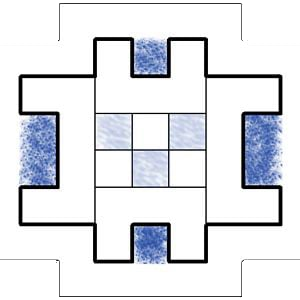
\includegraphics[width=\textwidth]{../pleonex.png}
    \end{column}
    \end{columns}

    \vfill
    \setlength{\leftmargini}{0em}
    \begin{itemize}
        \item Graduado en Ingeniería de Tecnologías de Telecomunicación
        \item Miembro de la Rama Estudiantil de IEEE para la UGR
        \item > 6 años en el mundo del ROM Hacking
    \end{itemize}
\end{frame}

\begin{frame}{Mis proyectos}
    \setlength{\leftmargini}{0em}
    \begin{columns}
    \begin{column}{0.4\textwidth}
        \Large Tinke
        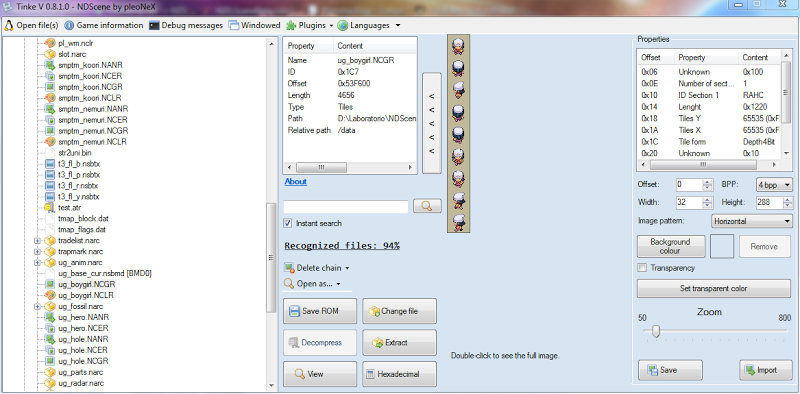
\includegraphics[width=\textwidth]{tinke_preview.png}
    \end{column}
    \begin{column}{0.6\textwidth}
        \Large Ninokuni \\ El Mago de las Tinieblas
    \end{column}
    \end{columns}

    \vfill
    \small
    \begin{columns}
    \begin{column}{0.3\textwidth}
        Libgame \\
        NinoImager \\
        NerdFontTerminatoR
    \end{column}
    \begin{column}{0.3\textwidth}
        Modime \\
        NinoDrive \\
        Sadler
    \end{column}
    \begin{column}{0.3\textwidth}
        NinoPatcher \\
        Zerum \\
        NinoDecompiler
    \end{column}
    \end{columns}

    \vfill
    \begin{columns}
    \begin{column}{0.5\textwidth}
        Final Fantasy: Four Heroes \\
        Bahamut \\
        Profesor Layton: London Life \\
        AAI
    \end{column}
    \begin{column}{0.5\textwidth}
        Shinning Force Feather \\
        Pokemon Conquest \\
        Inazuma Eleven 2 y 3 \\
        Hetalia
    \end{column}
    \end{columns}
\end{frame}

\subsection{El Big-Bang}
\begin{frame}{Érase una vez\ldots}
    \huge \centering
    La pregunta maldita
\end{frame}

\begin{frame}{¿Qué es un fichero?}
    \centering
    % TODO: Añadir foto de un fichero sin extension.
    \Huge ¿?
    \note<1>{Un fichero es simplemente un conjunto de bytes con significado.}
\end{frame}

\begin{frame}[t]{¿Qué hay dentro de un fichero?}
    \huge\centering
    ¿Qué hay para que veamos\ldots \\
    imágenes? \\
    vídeos? \\
    música? \\
    \vfill
    ¿Cómo lo vemos eso?
\end{frame}

\begin{frame}{La parte cruda de los archivos}
\end{frame}

\begin{frame}{Especificaciones}
\end{frame}

\begin{frame}{¿Qué hay dentro de un juego?}
\end{frame}

\begin{frame}{¿Y ahora? ¿Y la especificación?}
\end{frame}

\begin{frame}{This is ROM Hacking!}
\end{frame}

\subsection{TOC}
\begin{frame}{Contenido del curso}
    \centering
    \textbf{Introducción al ROM Hacking}
    \begin{enumerate}
        \item Edita tu primer videojuego
        \begin{enumerate}
            \item ¿Qué es ROM Hacking?
            \item Modifica un videojuego
        \end{enumerate}
        \item Formatos estándar en Nintendo DS
        \begin{enumerate}
            \item Textos
            \item Compresiones
            \item Imágenes
            \item Tipografías
            \item Audios
            \item Modelos 3D
        \end{enumerate}
        \item Programas de edición de ficheros
        \begin{enumerate}
            \item Crystal Tile
            \item New Super Mario Bros Level Editor
            \item Super Mario 64 DS Editor
            \item Pokémon
            \item Ninokuni
            \note<1>{TileMolester, DSLazy, CUE Compressors}
        \end{enumerate}
    \end{enumerate}
\end{frame}

\begin{frame}{¡Proyecto!}
    \Large
    \begin{wideitemize}
        \item Grupos de infinitas personas
        \item Traducción, edición, \textit{dumpeo}
        \item Trasversal al curso.
    \end{wideitemize}
\end{frame}

\begin{frame}{Futuros cursos}
    \begin{columns}
    \begin{column}{0.5\textwidth}
        \textbf{Desarrollo de herramientas de ROM Hacking}
        \begin{enumerate}
            \item Crear plugins para Tinke y Libgame.
            \item Crear programas editores de script, imágenes, \ldots
        \end{enumerate}
    \end{column}
    \hfill
    \begin{column}{0.5\textwidth}
        \textbf{ROM Hacking sobre ensamblador}
        \begin{enumerate}
            \item Aprender ensamblador
            \item Depurar juegos
            \item Modificar el código fuente de juegos
        \end{enumerate}
    \end{column}
    \end{columns}

\end{frame}
